\documentclass[a4paper,oneside,11pt]{article}
\usepackage{graphicx}
\usepackage{ tipa }
\usepackage{hyperref}
\usepackage{titling}
\usepackage{blindtext}
\usepackage{enumitem}
\usepackage{eurosym}
\usepackage{float}
\usepackage{listings}
\usepackage{tabularx}
\usepackage{alltt}
\usepackage[T1]{fontenc}
\usepackage{caption}
\usepackage{longtable}
\usepackage{changepage}
\usepackage{xcolor}
\captionsetup[figure]{}


\title{ATD}
\author{Daniele Montesi, Nicola Fossati, Francesco Sgherzi}
\date{\today}
\begin{document}
    \begin{titlingpage} 
        \begin{center}
            
\includegraphics[height=5cm]{assets/Logo_Politecnico_Milano.png}\\
            \vspace{4cm}
            \begin{huge} 
                \textbf{\thetitle} \\
            \end{huge}
            \vspace{0.3cm}
                    \begin{Large}
                \textit{Software Engineering 2 Project - TrackMe} \\
            \end{Large}
        \end{center}
         \textbf{v1.0} - 12/01/2019 \\

            \vspace{4cm}
             \begin{large}
            \textbf{Authors}
            \begin{itemize}
                \item Daniele Montesi - \textit{912980} 
                \item Nicola Fossati - \textit{915244}
                \item Francesco Sgherzi - \textit{915377}
            \end{itemize}
        \end{large}
    \end{titlingpage}
    \newpage
    \tableofcontents
    \newpage
    \section{Introduction}
    
        \subsection{Purpose}
            The main purpose of this document is to exhaustively describe the Data4Help main architecture, its parts and how they interact. There is also a chapter that covers the user interface.

The main recipients of this document are the project manager, developers and testers, but it can also be useful for further development reference and maintenance.
        \subsection{Scope}
            % To define the scope of the product we can use ``The World \& Machine'' approach by M. Jackson and P. Zave.
% We can define the real world entities that interact with the system (the World), the entities that belong to the system (the Machine) and the shared phenomena (the intersection of the two other sets).

% TODO: add image here

The \textit{The World and the Machine} approach is used in defining the scope of the project.
By defining the real world entities that interact with the system and the properties of the system itself we can determine the intersection between the two sets: the \textit{shared phenomena}.
\begin{center}
    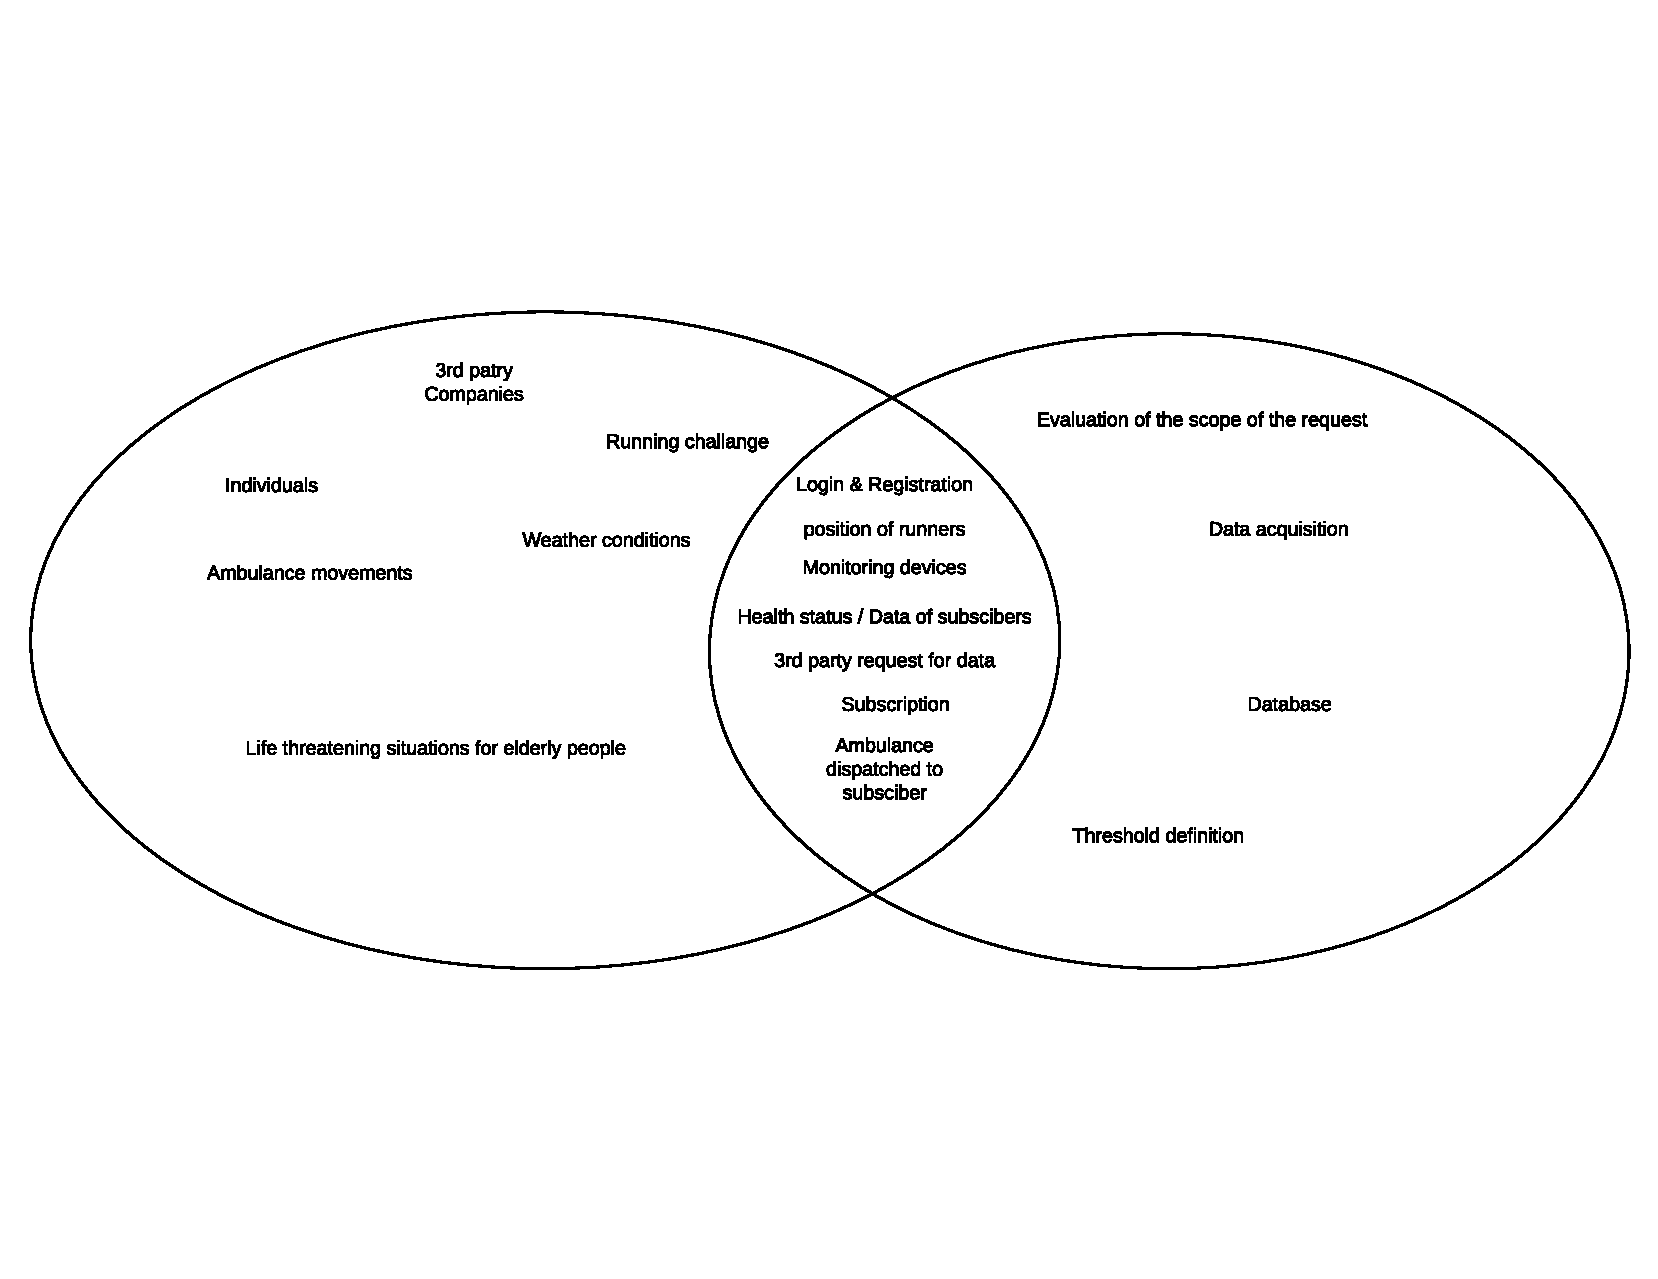
\includegraphics[height=8cm,keepaspectratio]{assets/twatm.pdf}
\end{center}

The system-to-be uses 3 components with different roles in order to work:
\begin{itemize}
    \item \textbf{Data4Help SmartWatch App}: Acquires the data from the smartwatch sensors (heart rate, sleep quality, position, phisical activities) and sends them via Bluetooth to the Data4Help Mobile App
    \item \textbf{Data4Help Mobile App}: Gathers data from the smartwatch, shows various statistics, and sends them to the Data4Help Core Database. Each user can choose which service subscribe to
    \item \textbf{Data4Help Website}: Gives third-party companies the ability to request data, either anonymized or user specific. Moreover, it allows run organizers to define the path of the run and the spectators to see the position of all runners on a map.
    \item \textbf{Data4Help Core}: is intended to connects all other components together providing the logic of the application. It is also responsible for the acceptance of all third-parties requests of data. It also evaluate health status of individuals deciding whether is at risk or not.
\end{itemize}

The list below shows the main goals the system should be able to accomplish:

\begin{itemize}
    \item \textbf{G1}: The system should be able to read sensor data from smart devices.
    \item \textbf{G2}: The system should be able to show acquired data via the Mobile App and the Website.
    \item \textbf{G3}: The system should allow users to register.
    \item \textbf{G4}: The system should allow companies to register.
    \item \textbf{G5}: The system should allow registered companies to request data either from specific individuals or from an anonymized group of individuals.
    \item \textbf{G6}: The system should allow users to accept or decline a company request for their specific data.
    \item \textbf{G7}: The system should provide a payment method to registered companies requesting user data. %eviterei di specificare payment system
    \item \textbf{G8}: The system should be able to communicate directly to ambulances.
    \item \textbf{G9}: The system should be able to react to the lowering of the health parameters below threshold in less than 5 seconds and send the position of the person to the ambulance system. 
    % \item \textbf{G10}: The system should should allow organizers to define the path for the run.
    \item \textbf{G10}: The system should be able to communicate interoperably with its services: \textit{AutomatedSOS} and \textit{Track4Run}
    \item \textbf{G11} The system should allow run organizers to register.
    \item \textbf{G12} If a run organizer is registered, it can define a run i.e. it can define the path that the participants should follow.
    \item \textbf{G13} A user should be able to enroll to a run.
    \item \textbf{G14} Spectators of a run should be able to see each participant's position on a map.
\end{itemize}

%A health data aggregator app that gives the user the ability to monitor all 

%is intended to offer all the functionalities of the service to the individuals, including heart rate monitoring, sleep monitoring




        \subsection{Definitions, Acronyms, Abbreviations}
            \input{chapters/1.3.DefinitionsAcronymsAbbreviations.tex}
            
        \subsection{Document structure}
        The document is divided into the following sections:
\begin{itemize}
    \item \textbf{Installation setup:} in this section the procedures and the steps followed in order to install and test the project will be discussed and explained, focusing on problem and incoherences found in the provided documents.
    \item \textbf{Acceptance test cases:} in this section all the tests run against the project will be discussed, relating them with the requirements / system goals described in the RASD and in the DD.
\end{itemize}
\newpage
    \section{Installation setup}
    
     We have followed the guide in the IT Document.
The guide was explained in details, even though, we had troubles in testing the system into a unique machine because of RAM limitation.
Probably it would have been better to have an instance of the server and of the database running online.


\subsection{Dependency installation}
We firstly installed the backend. To accomply this, on a Windows machine, you should first install ERLang and then install the RabbitMQ server.

After this, we proceed to install MySQL server and configure it following the guide linked in the IT Document.

The RabbitMQ server and MySQL server started automatically after the installation.

It is not clearly specified in the IDT but is also necessary to install a compatible version of Java and Maven (to run the tests). We installed, respectively, version \texttt{1.8.0\_191} and version \texttt{3.6.0}.

\subsection{Backend installation}
We simply extracted the precompiled version of the backend in an empty folder.
From there we launched each microservice executable, starting from \texttt{service-registry} and then all the other jar executables. 

Each service was launched using the command \texttt{java -jar *servicename*.jar}, exept the \texttt{api-gateway} which needs an additional command line parameter.
We think that this aspect was not stressed enough in the ITD; in fact in the first place we were not able to start the server correctly because we forgot the above mentioned configuration string.

\subsection{Frontend installation}
We installed the main Android app from the provided apk package in a new Android Emulator instance.
We then started the app, configured the IP of the server clicking on the app logo in the main screen.

To test the Bluetooth connection we installed the main app and the Bluetooth client in two different real devices.

The minimum Android version, as specified in the requirements, was 7.0 which made quite difficult to test since some of us had the version 6.0.
Moreover the app cannot be fully tested through the emulator since it exploit the Bluetooth connection, which cannot be emulated.
However, all the previous remarks were correctly explained in the ITD Document.





     
    
\newpage

    \section{Acceptance Test Cases}

    
The group has divided the requirements into:
\begin{itemize}
    \item Core requirements
    \item Goals and side requirements mapped
\end{itemize}

\noindent Here they are listed as reported in the RASD document:
\newline
\newline
\textbf{Core requirements}
\begin{itemize}
\item [{[R1]}] Allow a person to register into the system as a user by providing a username, a password, his credentials, his social security number and a consensus on the agreement

\item[{[R2]}] Allow a person or company to register into the system as a third party by providing an e-mail, a password, its credentials and a consensus on the agreement
\item[{[R3]}] A person cannot register as a user by inserting a username that has already been used in another successful registration process
\item[{[R4]}] A person cannot register as user by using the same social security number used in another successful registration process 

\item DELETED {[R5] A person cannot register as user by using the same credential used in another successful registration process}
\item DELETED {[R6] A person or company cannot register as third party into the system by using the same credentials used in another successful process}

\item[{[R7]}] A person or company cannot register as third party by using the same e-mail used in another successful registration process

\item[{[R8]}] Allow a person to log into the system as a user only if he has already registered as such
\item[{[R9]}] Allow a person or company to log into the system as a third party only if he has already registered as such
\end{itemize}

\newpage
\noindent The goals and mapped requirements are listed below: \\
\newline
\textbf{Goal reaching requirements}
\par


\begin{itemize}
\item [{[G1]}] Allow a user to access its own data
	\begin{itemize}
	\item[{[R10]}] If a user is logged-in, he is able to view its own data
	\end{itemize}
\item[{[G2]}] Allow a user to contribute to data sharing by providing information about his location and health status
	\begin{itemize}
	\item[{[R11]}] Allow a user to send its data to the system automatically when it is generated
	\end{itemize}
\item[{[G3 \& G4]}] Once the health parameters of a user have been observed 
below the threshold for the first time after one hour, an ambulance is sent to the user location. 
The time experienced between the moment in which the health parameters of a subscribed user are observed below the threshold and the time in which the emergency point is contacted is equal or less than 5 seconds
	\begin{itemize}
	\item[{[R12]}] When a user's health parameters has been observed below the threshold, an SOSCall is requested within 5 seconds
	\item[{[R13]}] All the automated SOS call are performed with devices of users whose health parameters are observed below a certain threshold
	\item[{[R14]}] An SOSCall can be requested only every minute
	\item[{[R15]}] An SOSCall is blocked if a previous one has already been accepted within one hour
	\item[{[R16]}] An SOSCall is implemented as an automated call by using an external API
	\item[{[R17]}] During an SOSCall, the GPS is set on high-precision
	\end{itemize}
\item[{[G5]}] Allow a user to participate in a run managed by third parties, as an athlete, if all starting conditions are satisfied.
	\begin{itemize}

	\item[{[R18]}] Allow a user to view a list of available runs, i.e. those that are still waiting to start 
	\item[{[R19]}] Allow a user to enroll in a run, after choosing it from the list, only before the expiration date by specifying his nickname
	\item[{[R20]}] Allow a user to unsubscribe from an enrolled run only before the expiration date
	\item[{[R21]}] If, after the expiration date, the number of participants is less than the minimum number defined by the organizer, then it is impossible to start the run.
	\item[{[R22]}] If the run cannot start due to minimum number of participants unsatisfied, then the enrolled runners are notified.
	\end{itemize}
\item[{[G6]}] Allow spectators (i.e. user) to see on real-time the "correct" positions of all athletes taking part in a run, with at most 15 meters of radius error
	\begin{itemize}
	\item[{[R23]}] Every athlete participating on a run, only on this specific occasion, shares continuously (i.e. each ten seconds) its position through a device
	\item[{[R24]}] Allow a spectator to see on a map the real-time position of every athlete in a specific run
	\end{itemize}
\item[{[G7]}] The maximum time to accept an individual request from any third party is 30 days; after that, the request will expire
	\begin{itemize}
	\item[{[R25]}] Once the time elapsed from sending request is greater than 30 days, then the request will be deleted from the system
	\end{itemize}
\item[{[G8 \& G9]}] Allow a user to accept or refuse a request from third parties. Allow a user to block requests made by a specific third party and all the pending requests will be refused: this action is possible only when the user has already refused one request made
by the customer that he is intending to block. 
	\begin{itemize}
	\item[{[R26]}] Allow a user to receive individual requests about data sharing from third parties
	\item[{[R27]}] Allow a user to view a list of pending requests
	\item[{[R28]}] Allow a user to accept or refuse a request from the list of pending request
	\item[{[R29]}] Allow a user to block requests from a defined third party, after having refused a request made by the customer
	involved in the block.
	\item[{[R46]}] When a request it is blocked, the other requests sent by the same Third party to the same user are refused.
	\end{itemize}	
\item[{[G10]}] Allow spectators and runners to see the leaderboard, when a run is completed
	\begin{itemize}
	\item[{[R30]}] Allow an organizer to close the run (when it is terminated)
	\item[{[R31]}] After a run is closed, the leaderboard is shown to the spectators and runners
	\item[{[R32]}] After a day is elapsed from the date of the race, if the run is not closed the application will automatically close it.
	\end{itemize}
\item[{[G11]}] Allow organizers (i.e. third parties) to set up a run, by defining its name, its path, date, start time, expiration date, and the minimum number of participants
	\begin{itemize}
	\item[{[R33]}] Allow a third party to see a map of the world with feasible paths
	\item[{[R34]}] Allow a third party to publish a race by providing an unique name, a feasible and a non-overlapping path (non-overlapping with other races of the same date), a date, a start time, a brief description, an expiration date for subscription and a minimum number of participants
	\item[{[R45]}] Allow a third party to manage its run by giving him a list of its managed race
	\end{itemize}
\item[{[G12]}] Allow a third party to access data specified in a request if the user accepts the request or if he accepted one or more requests from the same third party that provided access to the same data 
	\begin{itemize}
	\item[{[R35]}] If an individual request is accepted, then the third party who has made the request can access the data specified in the request
	\item[{[R36]}] For each piece of individual data accessible by a third part customer, exists an accepted request regarding it, performed by the same third party 
	\item[{[R37]}] Allow a user to accept or refuse request given by third parties
	\item[{[R38]}] Allow a third party to send individual requests to users by providing the user's social security number and a brief motivation
	\end{itemize}
\item[{[G13]}] Allow a third party to access statistical and anonymized data if and only if the number of individual involved is greater than 1000. This is satisfied after the request is approved  
	\begin{itemize}
	\item[{[R39]}] A group request is accepted if the aggregated data specified in the request is accessible to the third party who performed the demand
	\item[{[R40]}] Group requests are accepted if and only if the number of user involved is greater than 1000
	\item[{[R41]}] Aggregated data is accessible to a third party if an accepted aggregated data that request that data exists
	\item[{[R42]}] Allow a third party to send group request to the system regarding data about many users
	\end{itemize}
\item[{[G14]}] Allow a third party to subscribe to non-existing data. They will have access to them, after the data is generated. 
	\begin{itemize}
	\item[{[R43]}] Allow a third party to express a data request on future data
	\item[{[R44]}] A third party can have access to non-existing aggregated data regarding future information if and only if the number of people involved will be greater than 1000
	\end{itemize}
\end{itemize}


\newpage

\subsection{Test cases}
\subsubsection{Core requirements}

  \begin{adjustwidth}{1cm}{}
        \begin{longtable}{|c|p{0.7 \textwidth}|}
            \hline
            \textbf{Requirements} & \textbf{Notes} \\
            \hline
            \textbf{\textcolor{green}{R1}} & Ok, tested opening the app and clicking "Register" button and filling up the form in "User". \\
            \hline
            \textbf{\textcolor{green}{R2}} & Ok, tested opening the app and clicking "Register" button and filling up the form in "Third Party".   \\
            \hline
            \textbf{\textcolor{green}{R3}} & Ok, but wrong error description.  \\
                    \hline
            \textbf{\textcolor{green}{R4}} & Ok, by registering an user with the same SSN of a previous one. \\
                        \hline
            \textbf{\textcolor{green}{R7}} & Ok, we tried to register a Third Party with the same email of another registered Third Party.  \\
                        \hline
            \textbf{\textcolor{green}{R8}} & Ok, tested creating new accounts and then trying to log in. \\
                        \hline
            \textbf{\textcolor{green}{R9}} & Ok, tested creating new account and then trying to log in.\\
                        \hline

        \end{longtable}
    \end{adjustwidth}

\subsubsection{G1: Access to user's data}
  \begin{adjustwidth}{1cm}{}
        \begin{longtable}{|c|p{0.7 \textwidth}|}
            \hline
            \textbf{Requirements} & \textbf{Notes} \\
            \hline
            \textbf{\textcolor{green}{R10}} & Ok, tested after logging in with a user and sending data via the companion bluetooth app with another smarthpone. Then the user can click to "History" tab and see all acquired data.  \\
            \hline
        
        \end{longtable}
    \end{adjustwidth}
    
\subsubsection{G2: Load data automatically into the server}
  \begin{adjustwidth}{1cm}{}
        \begin{longtable}{|c|p{0.7 \textwidth}|}
            \hline
            \textbf{Requirements} & \textbf{Notes} \\
            \hline
            \textbf{\textcolor{yellow}{R11}} & Partially, tested logging in using another device with the same username and password of an already existing user and seeing data being in the history. However, location data are not available. \\
            \hline
            
            
        \end{longtable}
    \end{adjustwidth}
    
\subsubsection{G3 \& G4: Ambulance call}
  \begin{adjustwidth}{1cm}{}
        \begin{longtable}{|c|p{0.7 \textwidth}|}
            \hline
            \textbf{Requirements} & \textbf{Notes} \\
            \hline
            \textbf{\textcolor{green}{R12}} & Ok, tested inserting data lower to the treshold (1 bpm). The call is performed almost instantaneously.  \\
            \hline
            \textbf{\textcolor{green}{R13}} & Ok, identical to R12, tested inserting data lower to the treshold (1 bpm). The call is performed almost instantaneously.  \\
            \hline
            \textbf{\textcolor{green}{R15}} & Ok, tested after a call, tried to send twice the same data lower the treshold after 30m, but the call didn't work. Trying after more than one hour results in a correct call being dispatched.  \\
            \hline
            \textbf{\textcolor{green}{R17}} & Automatically done by the Android OS when performing an emergency call.  \\
            \hline            
            
        \end{longtable}
    \end{adjustwidth}
    
\subsubsection{G8 \& G9: User manages a request from third party}
  \begin{adjustwidth}{1cm}{}
        \begin{longtable}{|c|p{0.7 \textwidth}|}
            \hline
            \textbf{Requirements} & \textbf{Notes} \\
            \hline
            \textbf{\textcolor{green}{R26}} & Ok, tested generating a new individual request.  \\
            \hline
            \textbf{\textcolor{green}{R27}} & Ok, tested after having generated a requests and checking  the pending request section. \\
            \hline
            \textbf{\textcolor{green}{R28}} & Ok, tested after having generated a requests and then letting the user reject it. \\
            \hline
            \textbf{\textcolor{green}{R29}} & Ok, tested after having generated a requests and then letting the user reject it. After that the Third Party isn't allowed to send individual requests to the user anymore. \\
            \hline
            \textbf{\textcolor{green}{R46}} & Ok, tested like R26 and R29.  \\
            \hline            
            
            
        \end{longtable}
    \end{adjustwidth}
    
\subsubsection{G12: Third party access to a specific user data}
  \begin{adjustwidth}{1cm}{}
        \begin{longtable}{|c|p{0.7 \textwidth}|}
            \hline
            \textbf{Requirements} & \textbf{Notes} \\
            \hline
            \textbf{\textcolor{red}{R35}} & We couldn't test it as the app stopped responding when tapping on the "Download" icon.
            However, after contacting the developers they promptly released an update for the app that allowed us to download users' data. Still, the data concerning the position of the user aren't available.\\
            \hline
            \textbf{\textcolor{yellow}{R36}} & Like R35. However, after the update, we checked that this consistency constrain is maintained \\
            \hline
            \textbf{\textcolor{green}{R37}} & Ok, tested by sending an individual request for data and letting the user accept or refuse it. The Third Party user correctly displays the status of the request  \\
            \hline
            \textbf{\textcolor{green}{R38}} & Ok, tested by sending inserting, in the body of the request, the correct SSN of the user and a motivation. User correctly sees the request and the motivation and is able to accept or refuse it.  \\
            \hline
            
            
            
        \end{longtable}
    \end{adjustwidth}
    
\subsubsection{G13: Company access to group of anonimyzed data}
  \begin{adjustwidth}{1cm}{}
        \begin{longtable}{|c|p{0.7 \textwidth}|}
            \hline
            \textbf{Requirements} & \textbf{Notes} \\
            \hline
            \textbf{\textcolor{green}{R39}} & Ok, tested performing a query. \\
            \hline
            \textbf{\textcolor{green}{R40}} & Ok, tested by performing a request on an almost empty database and testing that the query was rejected.  \\
            \hline
            \textbf{\textcolor{green}{R41}} & Ok, tested performing a query on an almost empty database and testing that the data weren't accessible by the company (that is, that specific item shows a tag \textcolor{red}{REFUSED} and it is not possible to download the data as the "Download" icon is missing )  \\
            \hline
            \textbf{\textcolor{green}{R42}} & Ok, tested by performing a query on an almost empty database. Even if the query was rejected (wasn't possible to download users' data) it was still saved.  \\
            \hline
            
            
            
        \end{longtable}
    \end{adjustwidth}

\subsection{Unit and integration tests}
\subsubsection{Android app}
We also run other group's tests against the Android application in emulator, as described in the Installation section of the ITD. We were not able to run all the tests correctly, even after contacting the other group for clarifications, possibly due to some configuration mismatch in the emulator.

\noindent\textit{Tests in 'com.trackme.trackmeapplication': 24 total, 4 error, 20 passed}

\paragraph{localdb.database.AppDatabaseTest}

  \begin{adjustwidth}{1cm}{}
        \begin{longtable}{|p{0.5 \textwidth}|p{0.2 \textwidth}|p{0.2 \textwidth}|}
            \hline
            \textbf{Test} & \textbf{Result} & \textbf{Time} \\
            \hline
            insertEmergencyCall & \textcolor{green}{passed} & 105 ms \\
            \hline
            insertPositionData &  \textcolor{green}{passed} & 103 ms\\
            \hline
            insertPositionDataFail DueToNullValue & \textcolor{green}{passed} & 138ms \\
            \hline
            getNumberOfRecentCalls & \textcolor{green}{passed} & 127 ms\\
            \hline
            deleteAllPositionData & \textcolor{green}{passed} &  153 ms\\
            \hline
            deleteAllHealthData &  \textcolor{green}{passed}  &  103 ms\\
            \hline
            deleteAllRecentCalls & \textcolor{green}{passed} & 128 ms\\
            \hline
            insertHealthData &  \textcolor{green}{passed} & 52 ms\\
            \hline
            insertHealthDataFail DueToNullValue & \textcolor{green}{passed} & 77 ms \\
            \hline
        
        \end{longtable}
    \end{adjustwidth}
    
\paragraph{service.health.HealthDataCallbackTest}

  \begin{adjustwidth}{1cm}{}
        \begin{longtable}{|p{0.5 \textwidth}|p{0.2 \textwidth}|p{0.2 \textwidth}|}
            \hline
            \textbf{Test} & \textbf{Result} & \textbf{Time} \\
            \hline
            handleMessageCorrect WithRecentEmergencyCall & \textcolor{green}{passed} & 180 ms \\
            \hline
            handleMessageThrow InvalidHealthDataException DueToLocation &  \textcolor{green}{passed} & 75 ms\\
            \hline
            handleMessageThrow TimeExceptionDueToLocation & \textcolor{green}{passed} & 154 ms \\
            \hline
            handleMessageThrow InterruptedExceptionDueToLocation & \textcolor{green}{passed} & 102 ms\\
            \hline
            handleMessageCorrect WithSuccessCall & \textcolor{green}{passed} &  103 ms\\
            \hline
            handleMessage ThrowEmergencyNumberNotFoundException DueToLocation &  \textcolor{green}{passed}  &  76 ms\\
            \hline
            handleMessageGoodHealthData WithoutRecentEmergencyCall & \textcolor{green}{passed} & 77 ms\\
            \hline
            handleMessageGoodHealthData WithRecentEmergencyCall &  \textcolor{green}{passed} & 78 ms\\
            \hline
        
        \end{longtable}
    \end{adjustwidth}
    
    
\paragraph{HealthServiceHelperImplTest\$TestWithPermissionGranted}

  \begin{adjustwidth}{1cm}{}
        \begin{longtable}{|p{0.5 \textwidth}|p{0.2 \textwidth}|p{0.2 \textwidth}|}
            \hline
            \textbf{Test} & \textbf{Result} & \textbf{Time} \\
            \hline
            makeEmergencyCall & \textcolor{red}{failed}: java. util. concurrent. TimeoutException: No last location available  & 3.0 s \\
            \hline
        
        \end{longtable}
    \end{adjustwidth}
    
    
\paragraph{HealthServiceTest\$IntegrationTesting}

  \begin{adjustwidth}{1cm}{}
        \begin{longtable}{|p{0.5 \textwidth}|p{0.2 \textwidth}|p{0.2 \textwidth}|}
            \hline
            \textbf{Test} & \textbf{Result} & \textbf{Time} \\
            \hline
            testDoubleConsecutiveCall & \textcolor{red}{failed}: java. lang. IllegalArgumentException: Provider "gps" unknown   & 2.75 s \\
            \hline
            testMakeCallPerformance & \textcolor{red}{failed}: java. lang. IllegalArgumentException: Provider "gps" unknown  & 2.34 s \\
            \hline
        
        \end{longtable}
    \end{adjustwidth}
    
    
\paragraph{HealthServiceTest\$TestWithPermissionGranted}

  \begin{adjustwidth}{1cm}{}
        \begin{longtable}{|p{0.5 \textwidth}|p{0.2 \textwidth}|p{0.2 \textwidth}|}
            \hline
            \textbf{Test} & \textbf{Result} & \textbf{Time} \\
            \hline
            getUserLocation HasLastLocation & \textcolor{red}{failed}: java. util. concurrent. TimeoutException: No last location available     & 2.79 s \\
            \hline
            getEmergencyRoom NumberWrongCountryCode & \textcolor{green}{passed} & 3.48 s \\
            \hline
            getEmergencyRoom NumberForItaly & \textcolor{green}{passed}  & 2.97 s \\
            \hline
            getEmergencyRoom NumberForAfghanistan & \textcolor{green}{passed}  & 2.97 s \\
            \hline
        
        \end{longtable}
    \end{adjustwidth}
    
    
\noindent\textit{Tests util in app: 29 total, 29 passed}
\paragraph{HealthDataInspectorImplTest}

\begin{adjustwidth}{1cm}{}
        \begin{longtable}{|p{0.5 \textwidth}|p{0.2 \textwidth}|p{0.2 \textwidth}|}
            \hline
            \textbf{Test} & \textbf{Result} & \textbf{Time} \\
            \hline
            isGraveConditionInvalidData DueToNullValue1 & \textcolor{green}{passed} & 4 ms \\
            \hline 
            isGraveConditionInvalidData DueToNullValue2 & \textcolor{green}{passed} & 1 ms \\
            \hline 
            isGraveConditionInvalidData DueToNullValue3 & \textcolor{green}{passed} & 0 ms \\
            \hline 
            isGraveConditionInvalidData DueToNullValue4 & \textcolor{green}{passed} & 0 ms \\
            \hline 
            isGraveConditionInvalidData DueToNullValue5 & \textcolor{green}{passed} & 1 ms \\
            \hline 
            isGraveConditionInvalidData DueToNullValue6 & \textcolor{green}{passed} & 0 ms \\
            \hline 
            isGraveConditionInvalidData DueToNullValue7 & \textcolor{green}{passed} & 0 ms \\
            \hline 
            isGraveConditionInvalidData DueToNullValue8 & \textcolor{green}{passed} & 0 ms \\
            \hline 
            isGraveConditionInvalidData DueToNullValue9 & \textcolor{green}{passed} & 0 ms \\
            \hline 
            isGraveConditionInvalidData DueToBloodOxygen LevelLess0 & \textcolor{green}{passed} & 0 ms \\
            \hline
            isGraveConditionInvalid DateSinceTimestamp BeforeBirthDate & \textcolor{green}{passed} & 1 ms \\
            \hline
            isGraveConditionInvalid DataDueToPressure & \textcolor{green}{passed} & 0 ms \\
            \hline
            isGraveConditionInvalid DataDueToBloodOxygen LevelGreater100 & \textcolor{green}{passed} & 0 ms \\
            \hline
        
        \end{longtable}
    \end{adjustwidth}


\paragraph{HealthDataInspectorImplTest\$ParameterTest}

\begin{adjustwidth}{1cm}{}
        \begin{longtable}{|p{0.5 \textwidth}|p{0.2 \textwidth}|p{0.2 \textwidth}|}
            \hline
            \textbf{Test} & \textbf{Result} & \textbf{Time} \\
            \hline
            isGraveCondition HeartBeatProblem[0] & \textcolor{green}{passed} & 0 ms \\
            \hline 
            isGraveCondition HeartBeatProblem[1] & \textcolor{green}{passed} & 0 ms \\
            \hline 
            isGraveCondition HeartBeatProblem[2] & \textcolor{green}{passed} & 0 ms \\
            \hline 
            isGraveCondition HeartBeatProblem[3] & \textcolor{green}{passed} & 0 ms \\
            \hline 
            isGraveCondition HeartBeatProblem[4] & \textcolor{green}{passed} & 0 ms \\
            \hline 
            isGraveCondition HeartBeatProblem[5] & \textcolor{green}{passed} & 1 ms \\
            \hline 
            isGraveCondition HeartBeatProblem[6] & \textcolor{green}{passed} & 0 ms \\
            \hline 
            isGraveCondition HeartBeatProblem[7] & \textcolor{green}{passed} & 0 ms \\
            \hline 
            isGraveCondition HeartBeatProblem[8] & \textcolor{green}{passed} & 0 ms \\
            \hline 
            isGraveCondition HeartBeatProblem[9] & \textcolor{green}{passed} & 0 ms \\
            \hline
            isGraveCondition HeartBeatProblem[10] & \textcolor{green}{passed} & 0 ms \\
            \hline
            isGraveCondition HeartBeatProblem[11] & \textcolor{green}{passed} & 0 ms \\
            \hline
            isGraveCondition HeartBeatProblem[12] & \textcolor{green}{passed} & 0 ms \\
            \hline
        
        \end{longtable}
    \end{adjustwidth}


\paragraph{ThresholdIntegerTest}

\begin{adjustwidth}{1cm}{}
        \begin{longtable}{|p{0.5 \textwidth}|p{0.2 \textwidth}|p{0.2 \textwidth}|}
            \hline
            \textbf{Test} & \textbf{Result} & \textbf{Time} \\
            \hline
            ThresholdIntegerTest.contains CheckBounds & \textcolor{green}{passed} & 0 ms \\
            \hline 
            ThresholdIntegerTest.construct ThresholdIntegerMaxLessThanMin & \textcolor{green}{passed} & 0 ms \\
            \hline 
            ThresholdIntegerTest.construct ThresholdIntegerMaxEqualMin & \textcolor{green}{passed} & 0 ms \\
            \hline 
        
        \end{longtable}
    \end{adjustwidth}
    
\subsubsection{Backend}
All test ran successfully, however, due to the sheer amount of them, being 307 in total, we decided to present their results grouped by microservices.

\begin{adjustwidth}{1cm}{}
        \begin{longtable}{|p{0.5 \textwidth}|p{0.2 \textwidth}|p{0.2 \textwidth}|}
            \hline
            \textbf{Test} & \textbf{Result} & \textbf{Time} \\
            \hline
            \texttt{api-gateway} & 89/89 \textcolor{green}{passed} & 5.01min \\
            \hline 
            \texttt{grouprequestservice} & 38/38 \textcolor{green}{passed} & 2.33min \\
            \hline 
           \texttt{individualrequestservice} & 86/86 \textcolor{green}{passed} & 5.36min \\
           \hline
           \texttt{sharedataservice} & 94/94 \textcolor{green}{passed} & 5.07min \\
           \hline 
        
        \end{longtable}
    \end{adjustwidth}
        
    \section{Effort spent}
        \begin{tabular}{l*{6}{c}r}
            Date & Nicola Fossati & Daniele Montesi & Francesco Sgherzi \\
            \hline
            14/01/2019 & 0 & 0 & 1   \\
            \hline
            17/01/2019 & 0 & 3 & 3   \\
            \hline
            18/01/2019 & 6 & 5 & 3   \\
            \hline
            19/01/2019 & 3 & 1 & 8   \\
            \hline
            Total & 0 & 0 & 0   \\
        \end{tabular}
\end{document}